\documentclass[]{book}
\usepackage{lmodern}
\usepackage{amssymb,amsmath}
\usepackage{ifxetex,ifluatex}
\usepackage{fixltx2e} % provides \textsubscript
\ifnum 0\ifxetex 1\fi\ifluatex 1\fi=0 % if pdftex
  \usepackage[T1]{fontenc}
  \usepackage[utf8]{inputenc}
\else % if luatex or xelatex
  \ifxetex
    \usepackage{mathspec}
  \else
    \usepackage{fontspec}
  \fi
  \defaultfontfeatures{Ligatures=TeX,Scale=MatchLowercase}
\fi
% use upquote if available, for straight quotes in verbatim environments
\IfFileExists{upquote.sty}{\usepackage{upquote}}{}
% use microtype if available
\IfFileExists{microtype.sty}{%
\usepackage[]{microtype}
\UseMicrotypeSet[protrusion]{basicmath} % disable protrusion for tt fonts
}{}
\PassOptionsToPackage{hyphens}{url} % url is loaded by hyperref
\usepackage[unicode=true]{hyperref}
\hypersetup{
            pdftitle={Omics Central},
            pdfauthor={Amrit Singh},
            pdfborder={0 0 0},
            breaklinks=true}
\urlstyle{same}  % don't use monospace font for urls
\usepackage{natbib}
\bibliographystyle{apalike}
\usepackage{longtable,booktabs}
% Fix footnotes in tables (requires footnote package)
\IfFileExists{footnote.sty}{\usepackage{footnote}\makesavenoteenv{long table}}{}
\usepackage{graphicx,grffile}
\makeatletter
\def\maxwidth{\ifdim\Gin@nat@width>\linewidth\linewidth\else\Gin@nat@width\fi}
\def\maxheight{\ifdim\Gin@nat@height>\textheight\textheight\else\Gin@nat@height\fi}
\makeatother
% Scale images if necessary, so that they will not overflow the page
% margins by default, and it is still possible to overwrite the defaults
% using explicit options in \includegraphics[width, height, ...]{}
\setkeys{Gin}{width=\maxwidth,height=\maxheight,keepaspectratio}
\IfFileExists{parskip.sty}{%
\usepackage{parskip}
}{% else
\setlength{\parindent}{0pt}
\setlength{\parskip}{6pt plus 2pt minus 1pt}
}
\setlength{\emergencystretch}{3em}  % prevent overfull lines
\providecommand{\tightlist}{%
  \setlength{\itemsep}{0pt}\setlength{\parskip}{0pt}}
\setcounter{secnumdepth}{5}
% Redefines (sub)paragraphs to behave more like sections
\ifx\paragraph\undefined\else
\let\oldparagraph\paragraph
\renewcommand{\paragraph}[1]{\oldparagraph{#1}\mbox{}}
\fi
\ifx\subparagraph\undefined\else
\let\oldsubparagraph\subparagraph
\renewcommand{\subparagraph}[1]{\oldsubparagraph{#1}\mbox{}}
\fi

% set default figure placement to htbp
\makeatletter
\def\fps@figure{htbp}
\makeatother

\usepackage{booktabs}
\usepackage{amsthm}
\makeatletter
\def\thm@space@setup{%
  \thm@preskip=8pt plus 2pt minus 4pt
  \thm@postskip=\thm@preskip
}
\makeatother

\title{Omics Central}
\author{Amrit Singh}
\date{2020-01-24}

\begin{document}
\maketitle

{
\setcounter{tocdepth}{1}
\tableofcontents
}
\chapter{Rationale}\label{rationale}

This project was developed in order to create a resource warehouse for
researchers analyze omics datasets of various types such as
transcriptomics, proteomcs, metabolomics. I expect this resource to grow
as others contribute to it. Think of it as an awesome-resource github
repo but in a bookdown format. However, since this book is meant as
documentation to the omics central web application, adding new methods
will require pull requests to the omics central web app repos
(omics-central-frontend, omics-central-backend and omics-central-docker)
and bookdown repos (omics-central-learn and omics-central-contribute).

The purpose of this book is not to copy, paste other works but to link
works by different authors in one place and explain concepts through the
lens of an omics researcher.

\chapter{Introduction}\label{intro}

\textbackslash{}TODO

\chapter{Data-types}\label{data-types}

\section{Microarrays}\label{microarrays}

\section{RNA sequencing}\label{rna-sequencing}

\section{Nanostring}\label{nanostring}

\section{Biocrates}\label{biocrates}

\section{Multiple Reaction
Monitoring}\label{multiple-reaction-monitoring}

\chapter{Exploratory Data Analysis}\label{eda}

\section{Principal Component
Analysis}\label{principal-component-analysis}

//TODO insert video of EDA using Omics Central here

\subsection{Method}\label{method}

\subsubsection{What is PCA?}\label{what-is-pca}

\begin{itemize}
\tightlist
\item
  method to turn a dataset with correlated variables into another
  dataset with linearly uncorrelated variables called principal
  components (PCs).
\end{itemize}

\subsubsection{Why is PCA useful?}\label{why-is-pca-useful}

\begin{itemize}
\tightlist
\item
  The first few PCs capture most of the variability in the data.
\item
  PCA can be used to visualize clustering patterns (samples or
  variables) in the data, determine relationships between samples (see
  Principal Component plot), between variables (see Correlation circle),
  between samples and variables (see Biplot).
\item
  PCA is also useful in determining the influece of covariates, both
  techincal (\emph{e.g.} batch effects) or biological (\emph{e.g.} sex).
\end{itemize}

\subsubsection{What is a principal component
(PC)?}\label{what-is-a-principal-component-pc}

\begin{itemize}
\tightlist
\item
  a PC is a weighted average of the original predictors,
  \textbf{PC}\textsubscript{\emph{i}} =
  \textbf{Xv}\textsubscript{\emph{i}}, where \textbf{X} is a centered
  matrix and \emph{i=1,\ldots{},n}.
\end{itemize}

\subsubsection{\texorpdfstring{What do the vector of weights
\textbf{v}\textsubscript{\emph{i}}
do?}{What do the vector of weights vi do?}}\label{what-do-the-vector-of-weights-vi-do}

\begin{itemize}
\tightlist
\item
  \emph{v\textsubscript{i}} maximizes the variance;
  \textbf{X\textsuperscript{T}X} and are called eigenvectors, weights or
  loadings.
\end{itemize}

\subsubsection{\texorpdfstring{How do I compute the vector of weights,
\emph{v\textsubscript{i}}?}{How do I compute the vector of weights, vi?}}\label{how-do-i-compute-the-vector-of-weights-vi}

\begin{itemize}
\tightlist
\item
  apply a factorization method called singular value decomposition
  (SVD). SVD decomposes a matrix X into a product of 3 matrices,
  \textbf{UDV\textsuperscript{T}}; \textbf{X}\textsubscript{\emph{np}} =
  \textbf{U}\textsubscript{\emph{nxp}} x
  \textbf{D}\textasciitilde{}\emph{pxp\textasciitilde{}} x
  \textbf{V\textsuperscript{T}}\textsubscript{\emph{pp}} or
  \textbf{X\textsuperscript{T}X} =
  \textbf{VD\textsuperscript{2}V\textsuperscript{T}}.
\item
  The columns of \textbf{V} are the weights/loadings for each principal
  component.
\item
  \textbf{D} is a diagnoal matrix where entry
  \textbf{D}\textsubscript{\emph{i,i}} is the standard deviation of the
  \emph{ith} principal component (PC).
\item
  Only the first \emph{k} PCs are needed to capture the majority of the
  variation in the high dimensional dataset (\emph{n}
  \textless{}\textless{} \emph{p} and \emph{k} \textless{}\textless{}
  \emph{p}); \textbf{X}\textsubscript{\emph{nk}} =
  \textbf{U}\textsubscript{\emph{nxk}} x
  \textbf{D}\textsubscript{\emph{pxk}} x
  \textbf{V\textsuperscript{T}}\textsubscript{\emph{nk}} such that
  \textbf{X}\textsubscript{\emph{nk}} \(\approx\)
  \textbf{X}\textsubscript{\emph{np}}.
\end{itemize}

\subsubsection{Why scale the data before applying
PCA?}\label{why-scale-the-data-before-applying-pca}

\begin{itemize}
\tightlist
\item
  The clinical variables are on different unit scales (\emph{e.g.} Age
  (years) \emph{vs.} Ejection fraction (\%)). Scaling makes the mean of
  each variable zero and the standard deviation one.
\end{itemize}

References\\
1. page 64-66 from ESL:
\url{https://web.stanford.edu/~hastie/ElemStatLearn/printings/ESLII_print10.pdf}\\
2. Wikipedia:
\url{https://en.wikipedia.org/wiki/Principal_component_analysis}

\subsection{Visualizations}\label{visualizations}

\subsubsection{Scree plot}\label{scree-plot}

\begin{itemize}
\tightlist
\item
  determine the proportion of variation explained by each principal
  component.
\end{itemize}

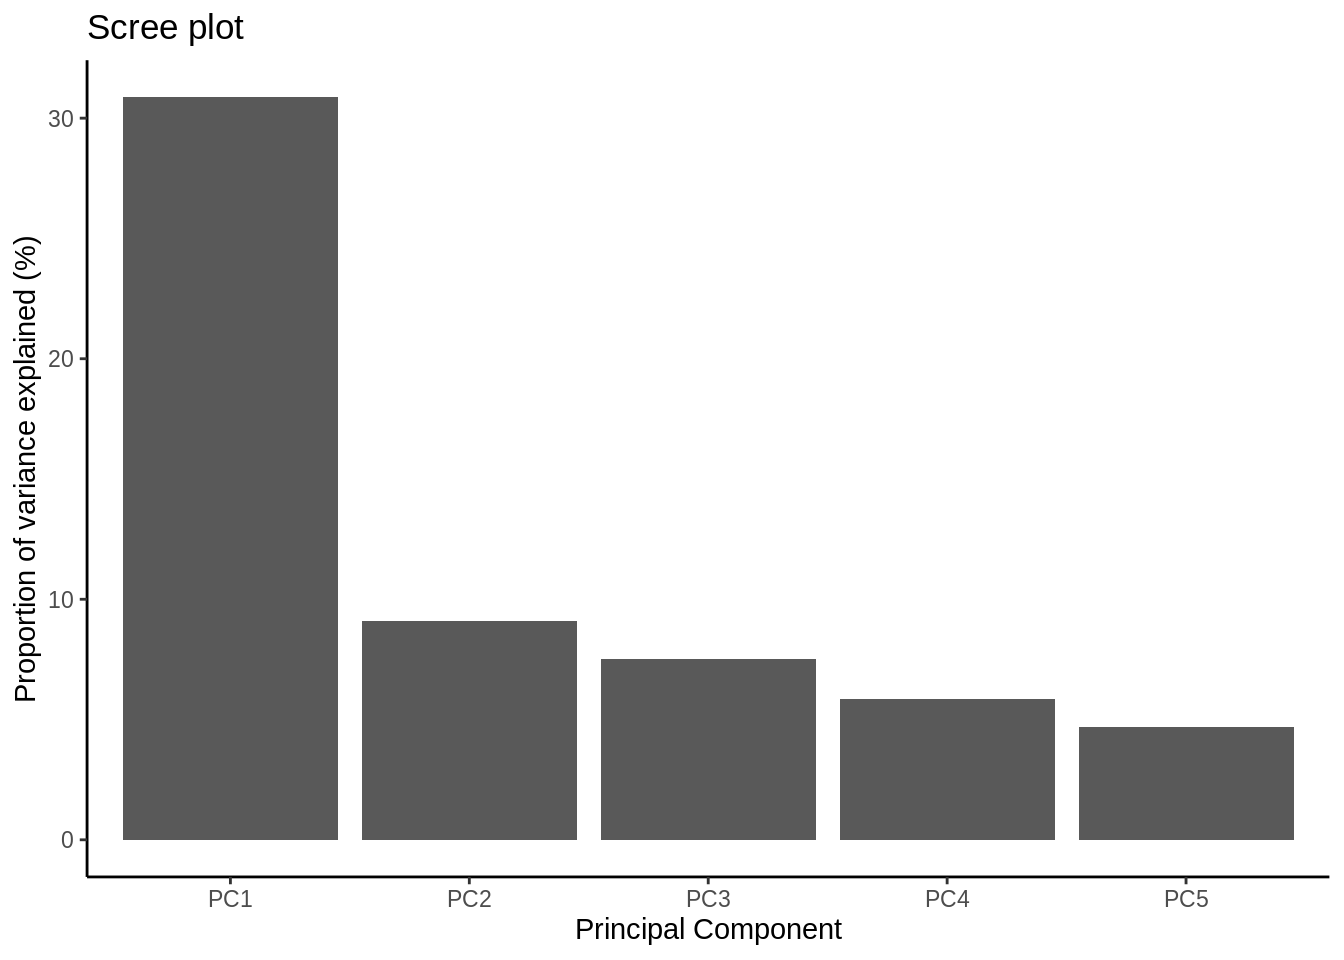
\includegraphics{bookdown-demo_files/figure-latex/unnamed-chunk-3-1.pdf}

\begin{quote}
The barplot depicts the proportion of variation that is captured by the
first five PCs; the first PC captures \textasciitilde{}30.9\% of the
variability in the dataset consisting of 65 variables.
\end{quote}

\subsubsection{Component plot}\label{component-plot}

\begin{itemize}
\tightlist
\item
  visualize the clustering of the samples and identify any clustering
  with respect to covariates of interest.
\end{itemize}

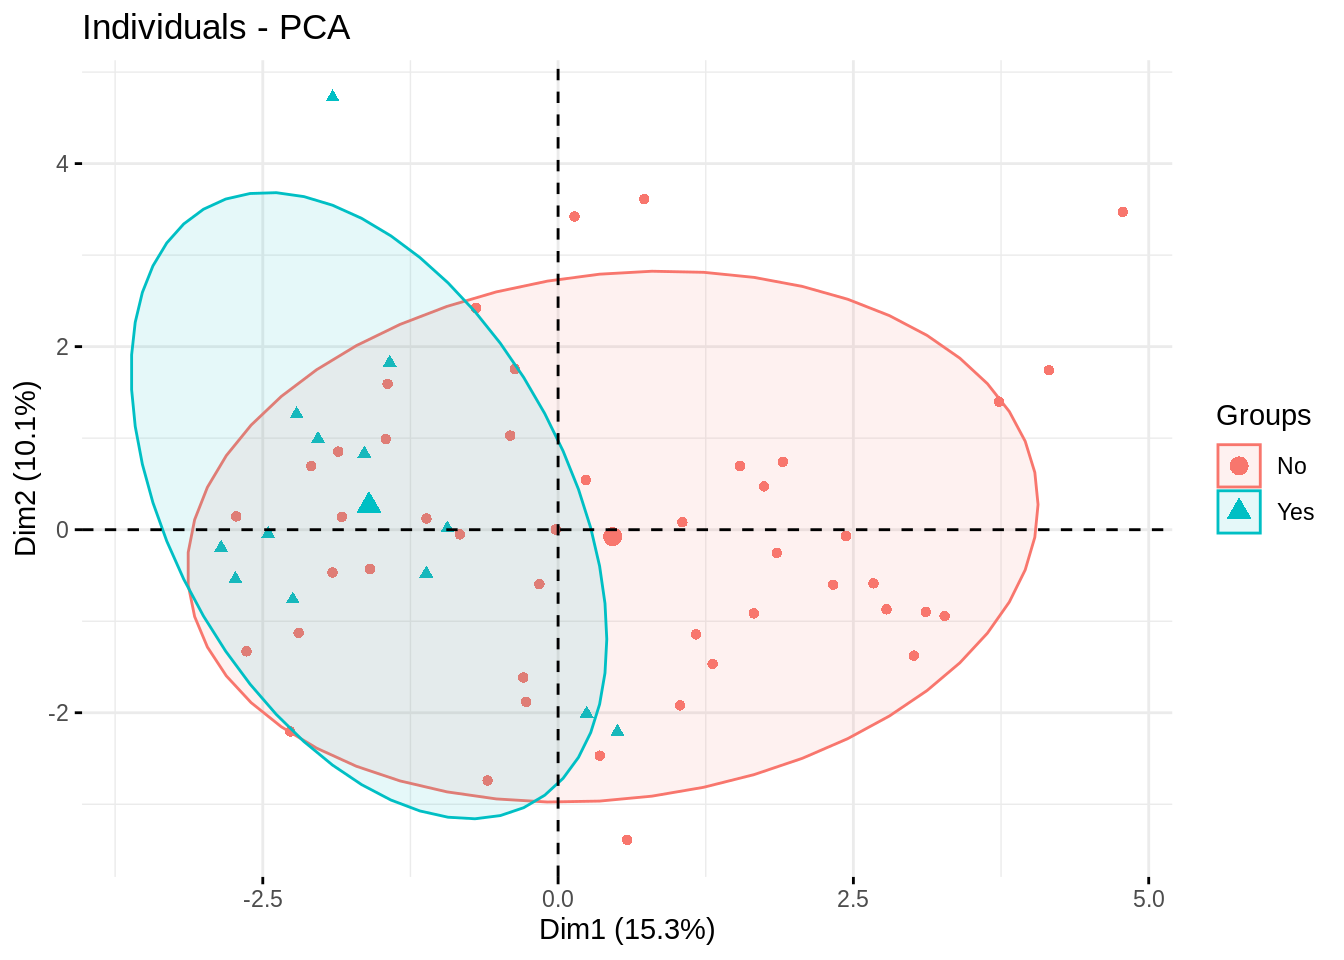
\includegraphics{bookdown-demo_files/figure-latex/unnamed-chunk-4-1.pdf}

\begin{quote}
The scatter plot above is a 2D depiction of a 65 (\# of clinical
variables) dimensional dataset. PC1 and PC2 together capture 40\% of the
variability in the clinical dataset. Some separation between the groups
of interest can be observed.
\end{quote}

\subsubsection{Correlation Circle}\label{correlation-circle}

\begin{itemize}
\item
  determine relationship between variables (based on the correlation
  between each variable and PCs).
\item
  the angle (\(\theta\)) between two vectors determines the correlation
  between the two variables:\\
\item
  \(\theta\)=0: postive correlation (corr=1)\\
\item
  0\textless{}\(\theta\)\textless{}90: postive correlation\\
\item
  \(\theta\)=90: zero correlation\\
\item
  90\textless{}\(\theta\)\textless{}180: negative correlation\\
\item
  \(\theta\)=180: negative correlation (corr=-1)
\end{itemize}

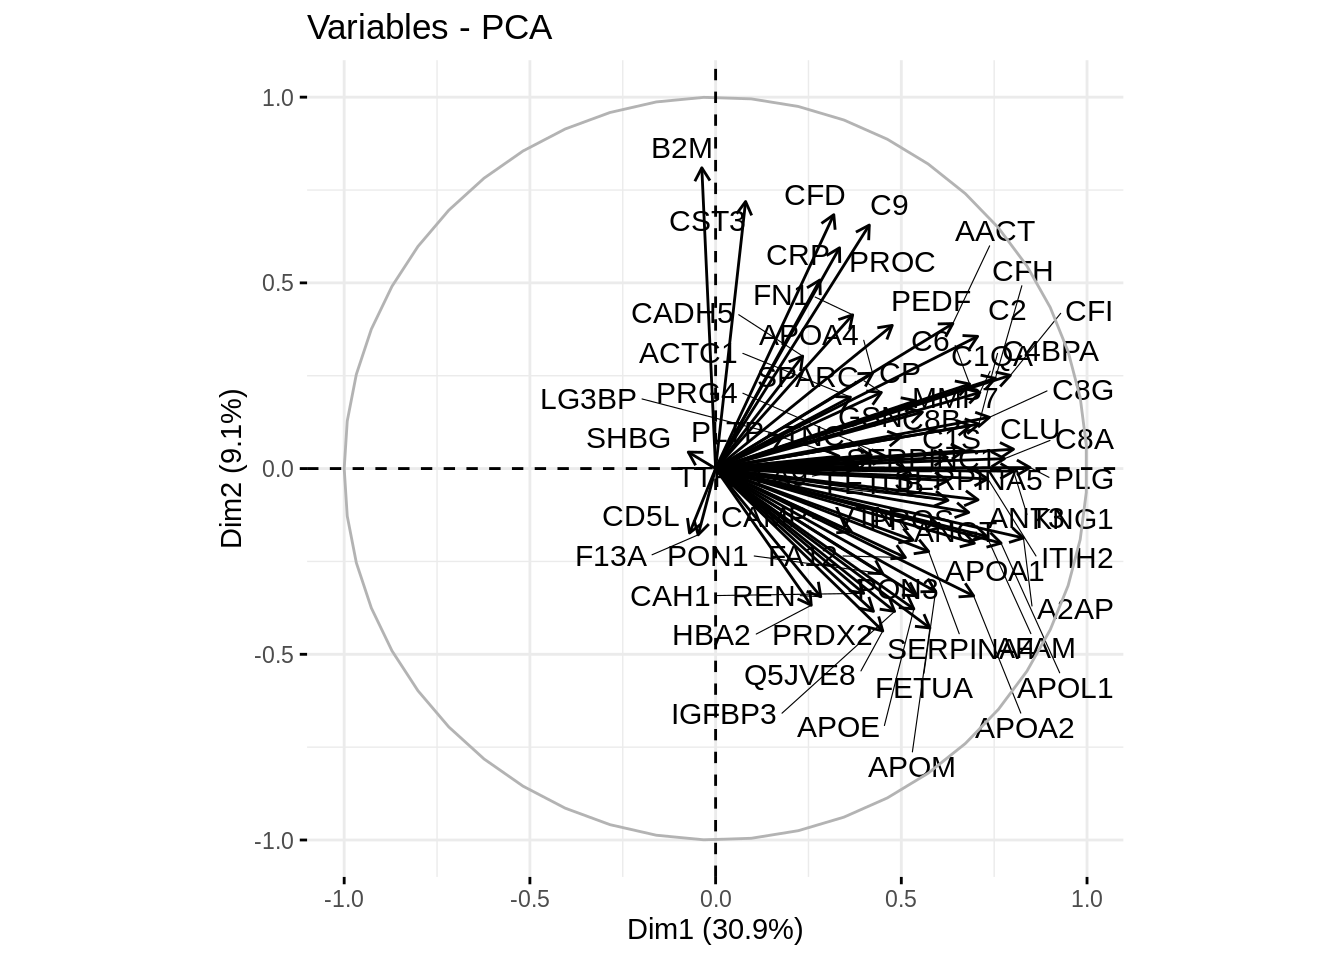
\includegraphics{bookdown-demo_files/figure-latex/unnamed-chunk-5-1.pdf}

\subsubsection{Correlation Circle (with a
cut-off)}\label{correlation-circle-with-a-cut-off}

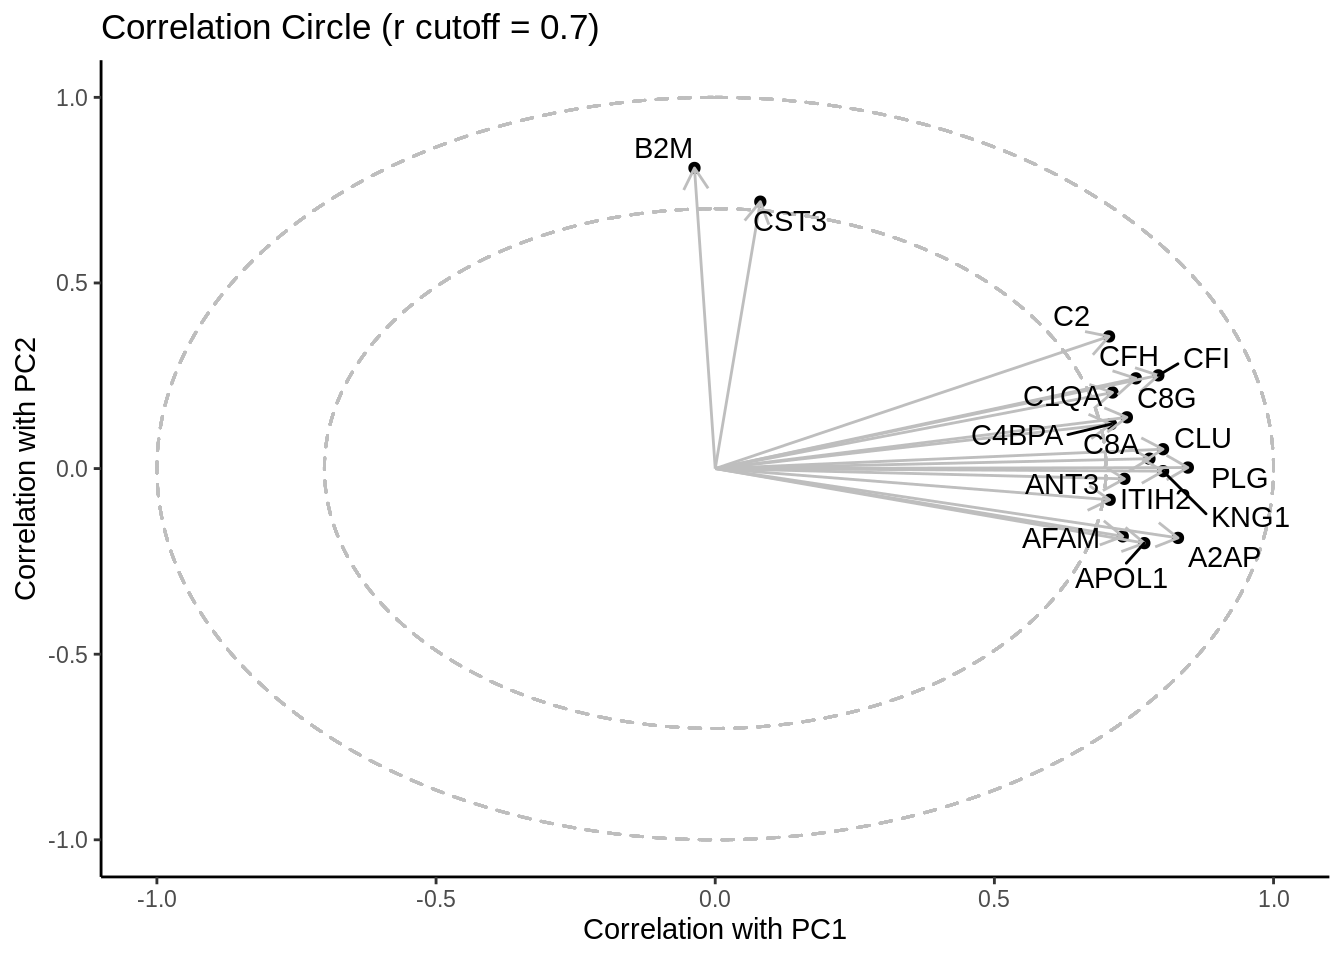
\includegraphics{bookdown-demo_files/figure-latex/unnamed-chunk-6-1.pdf}

\begin{quote}
The above plot only displays the variables if they have a correlation
greater than 0.5 with either PC1 or PC2. Ischemia and Statins are
positively correlated suggesting that patients with ischemia are likely
to be on statins. BNP (Brain Natriuretic Peptide) is positively
correlated with age and negatively correlated with Heart Rate.
\end{quote}

References\\
1. Figure 1 from BioData Mining volume 5, Article number: 19 (2012)\\
2. plotVar(): mixOmics R-library 3. fviz\_pca\_var(): factoextra
R-library

\subsubsection{Biplot}\label{biplot}

\begin{itemize}
\tightlist
\item
  superimpose the principal components with loadings vectors.
\end{itemize}

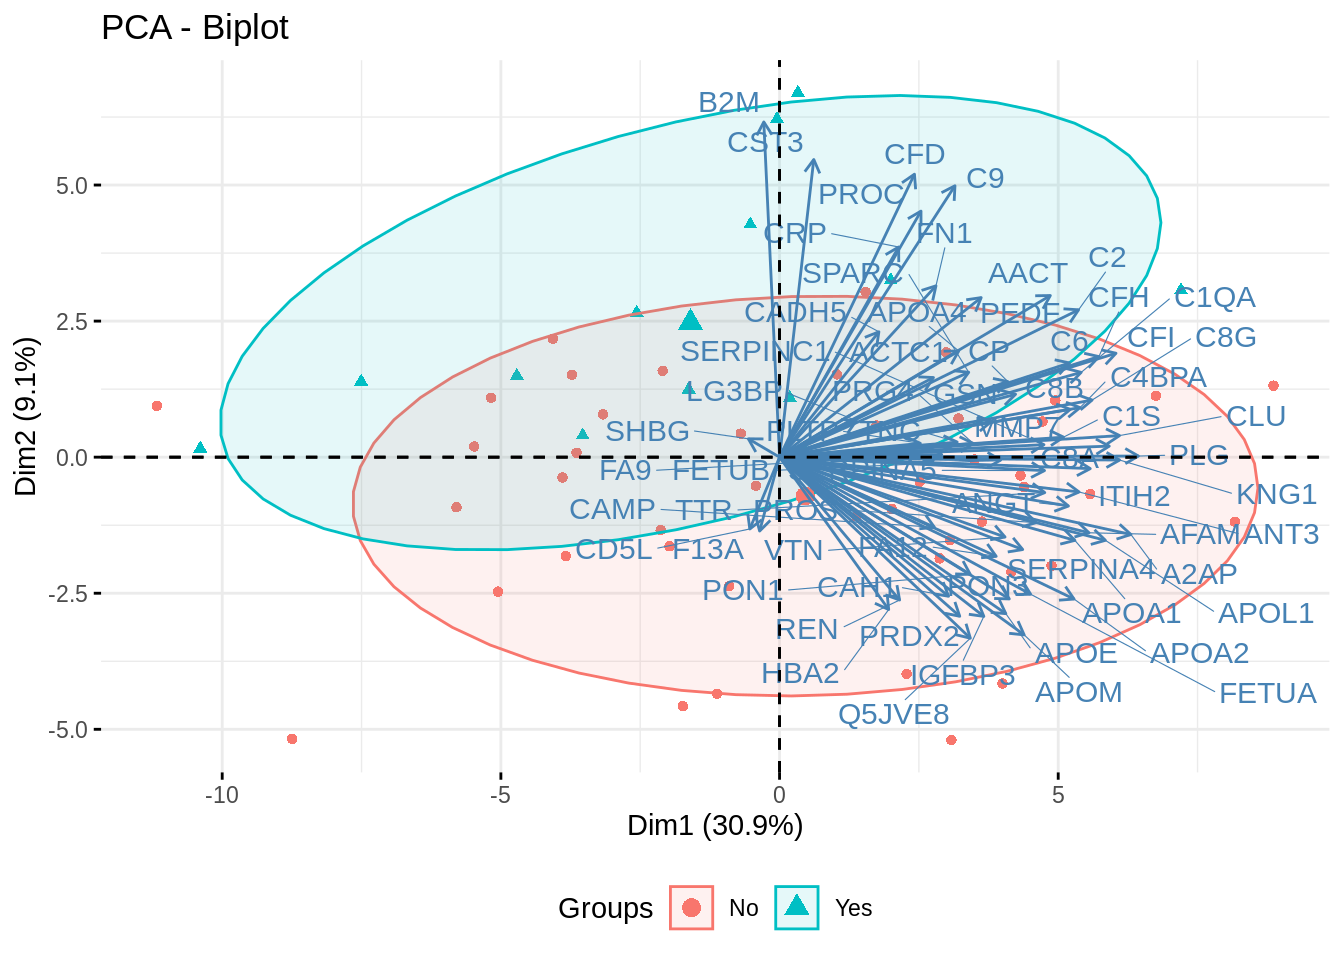
\includegraphics{bookdown-demo_files/figure-latex/unnamed-chunk-7-1.pdf}

\begin{quote}
Each arrow can be thought of as an axis. For example, BNP points to the
left which means that patients on the left (PC1 \textless{} 0) have
lower BNP levels than patients on the right (PC1 \textgreater{} 0).
Patients at the center (PC=1) have an average BNP level. Note that this
aligns well with the hospitalization status; \emph{ie.} patients on the
left are more likely to be hospitalized as compared to patients on the
right.
\end{quote}

References\\
1. ggbiplot(): \url{https://github.com/vqv/ggbiplot}\\
2. Biplot:
\url{https://stackoverflow.com/questions/6578355/plotting-pca-biplot-with-ggplot2}\\
3. biplot(): K. R. Gabriel (1971). The biplot graphical display of
matrices with application to principal component analysis. Biometrika,
58, 453--467. doi: 10.2307/2334381.\\
4. fviz\_pca\_biplot():
\url{http://www.sthda.com/english/wiki/fviz-pca-quick-principal-component-analysis-data-visualization-r-software-and-data-mining}

\subsubsection{Are the major sources of variation in the proteomics
dataset related to any demographics
variables?}\label{are-the-major-sources-of-variation-in-the-proteomics-dataset-related-to-any-demographics-variables}

\begin{itemize}
\tightlist
\item
  this is often answers by correlating the PCs with demographics
  variables such as batch or disease of interest.
\end{itemize}

\paragraph{Test the Pearson correlation between PCs and demographic
variables}\label{test-the-pearson-correlation-between-pcs-and-demographic-variables}

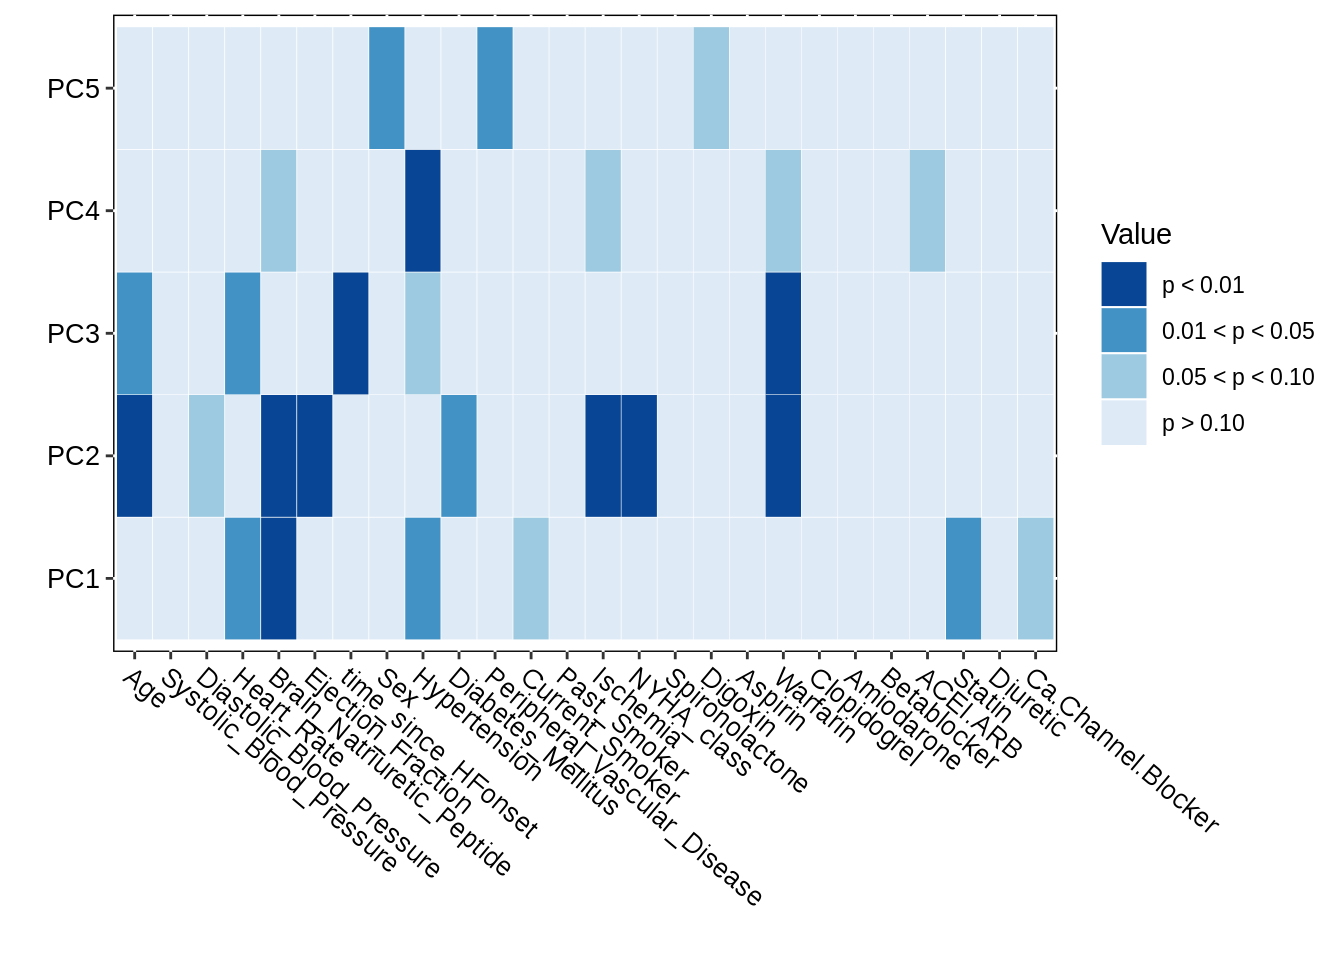
\includegraphics{bookdown-demo_files/figure-latex/unnamed-chunk-8-1.pdf}

\paragraph{Test the Spearman correlation between PCs and demographic
variables}\label{test-the-spearman-correlation-between-pcs-and-demographic-variables}

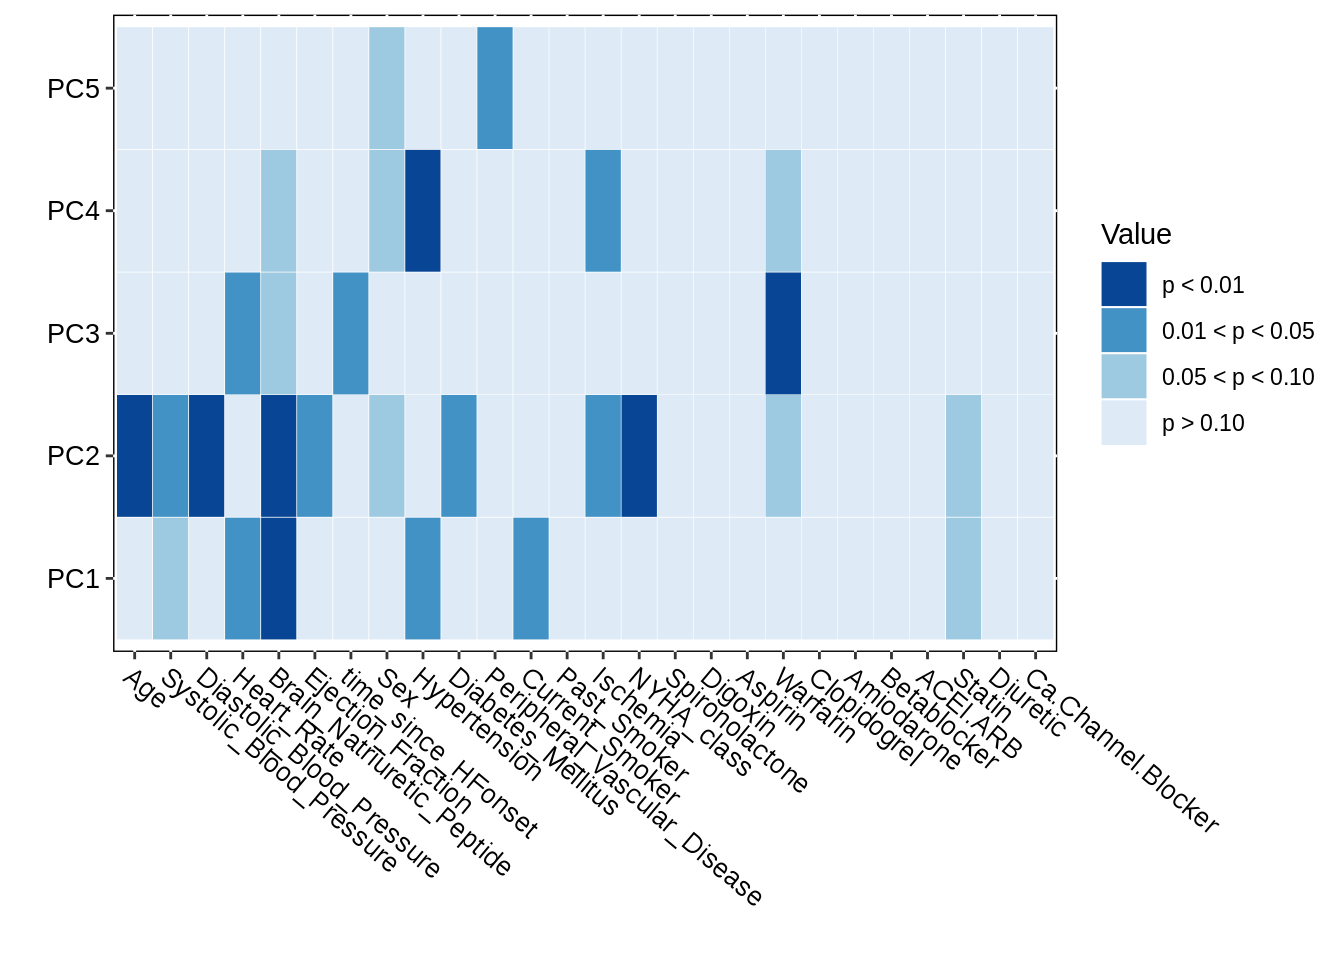
\includegraphics{bookdown-demo_files/figure-latex/unnamed-chunk-9-1.pdf}

\begin{quote}
The associtation between PC1 and BNP has a p-value of \textless{} 0.01
which supports the Biplot in which BNP was parallel to PC1 (x-axis).
\end{quote}

\textbf{WARNING}: This is only to be used for exploratory purposes and
not for inference since spurious correlations may arise.

\section{K-Means}\label{k-means}

\section{Hierarchical clustering}\label{hierarchical-clustering}

\section{Sample plots}\label{sample-plots}

\subsection{Sample correlation
heatmap}\label{sample-correlation-heatmap}

\subsection{Sample histograms}\label{sample-histograms}

\section{Variable plots}\label{variable-plots}

\chapter{References}\label{references}

\begin{enumerate}
\def\labelenumi{\arabic{enumi}.}
\tightlist
\item
  BioData Mining volume 5, Article number: 19 (2012)\\
\item
  PH525x series: \url{http://genomicsclass.github.io/book/}
\item
  mixOmics: \url{https://mixomicsteam.github.io/Bookdown}
\end{enumerate}

\chapter{Batch Correction}\label{batch-correction}

\section{ComBat}\label{combat}

\section{Surrogate Variable Analysis}\label{surrogate-variable-analysis}

\section{Model adjustment}\label{model-adjustment}

\section{References}\label{references-1}

\begin{enumerate}
\def\labelenumi{\arabic{enumi}.}
\tightlist
\item
  Batch effect simluations:
  \url{http://jtleek.com/svaseq/simulateData.html}
\item
  Surrogate Variable Analysis:
  \url{https://bioconductor.org/packages/release/bioc/vignettes/sva/inst/doc/sva.pdf}
\end{enumerate}

\chapter{Differential Expression Analysis}\label{diff-exp}

\section{Ordinary Least Squares}\label{ordinary-least-squares}

\section{LInear Models for MicroArrays and
RNA-Seq}\label{linear-models-for-microarrays-and-rna-seq}

\subsection{Robust LIMMA}\label{robust-limma}

\subsection{LIMMA VOOM}\label{limma-voom}

\section{Significance Analysis for Microarrays
(SAM)}\label{significance-analysis-for-microarrays-sam}

\section{cell-specific Analysis for Microarrays
(csSAM)}\label{cell-specific-analysis-for-microarrays-cssam}

\chapter{Network Analysis}\label{network-analysis}

\section{DINGO}\label{dingo}

\section{WGCNA}\label{wgcna}

\section{PANDA}\label{panda}

\section{BioNetStat}\label{bionetstat}

\chapter{Data Integration}\label{data-integration}

\section{Supervised}\label{supervised}

\subsection{DIABLO (SGCCDA)}\label{diablo-sgccda}

\subsection{Ensemble of glmnet
classifiers}\label{ensemble-of-glmnet-classifiers}

\subsection{DIABLO2 (sMB-PLSDA)}\label{diablo2-smb-plsda}

\section{Unsupervised}\label{unsupervised}

\subsection{PANDA}\label{panda-1}

\subsection{MOFA}\label{mofa}

\subsection{JIVE}\label{jive}

\subsection{SNF}\label{snf}

\chapter{Biological Enrichment}\label{bio-enrichment}

\section{Enrichr}\label{enrichr}

\section{SEAR}\label{sear}

\section{CAMERA}\label{camera}

\section{Network-based Gene Set
Analysis}\label{network-based-gene-set-analysis}

\chapter{Literature Mining}\label{lit}

\bibliography{book.bib,packages.bib}

\end{document}
